\section{Introduction}
Many distributed applications are routinely divided into fine-grained tasks that are executed simultaneously.
The key is to harness as many cores as possible in order to minimize completion time.
Recent advances in microservices and serverless computing (\eg, AWS Lambda~\cite{aws-lambda}, Azure Serverless Computing~\cite{azure-functions}, Google Cloud Functions~\cite{gcloud-functions}, and OpenFaaS~\cite{openfaas}), have led to impressive speedup of parallel applications, including video encoding~\cite{ExCamera}, video compression~\cite{sprocket}, and face recognition~\cite{cirrus}, by successfully employing thousands of CPU cores in parallel. Many applications could be accelerated even further if we break the application into tiny fine-grained fragments running on tens of thousands or even millions of cores. 
But, realistically, we quickly run into a minimum fragment size\shahbaz{didn't get this point, a bit unclear} caused by the time taken to invoke a remote code fragment. Today, even with the best microservices and fastest RPCs, it takes milliseconds to execute code remotely. This limits the degree of parallelism in a cloud datacenter, making it impractical to harness millions of cores for just a short time to complete a large job quickly.  So even though cloud data centers contain millions of CPU cores, any one application can only utilize a subset. We are interested in driving down the RPC time, to make it practical to harness many more CPUs simultaneously.

% Cloud data centers allow thousands of client applications to share millions of CPU cores.
% Many of these client applications harness CPU cores using {\em coarse}-grained parallelism, such as MapReduce~\cite{mapreduce-google}, Hadoop~\cite{apache-hadoop} and client-server web applications.
% Other, more specialized applications use {\em fine}-grained parallelism to employ hundreds of thousands of CPUs (\eg, search~\cite{barroso2003web}, HPC~\cite{ibm-hpc}).
% It is well-known to be difficult to write applications using fine-grained parallelism, and so the technique is generally reserved as a last resort, for when applications must respond quickly (\eg, search or ads), or must complete in a reasonable time (\eg, a large HPC physical simulation~\cite{changa, blue-gene-l, barnes-hut} or overnight ML training~\cite{tensorflow}).
% Recently, as applications have grown ever larger (\eg, mushrooming ML training data, big data analytics, and social media), the speed of individual cores has grown ever more slowly~\cite{hp-comp-arch}.
% Increased parallelism is inevitable.

In the limit, if we segment an application into its smallest, indivisible software modules, {\em and if communication is instantaneous}, then an application could complete in the execution time of the longest sequence of serially-dependent modules.
But, communication is not instantaneous---far from it. 
Many researchers have reported the (surprisingly) high communication latency between two cores, \eg, a request-response time of \SI{0.7}{ms}~\cite{eRPC, perfkit-grpc}.
Intuitively, if it takes \SI{0.7}{ms} to ask another CPU to execute a function, then it is only worth doing if we have more than \SI{0.7}{ms} of work to do; otherwise we might as well execute the code locally. 

For example, consider a physical simulation of one million objects, where each object needs to update its ten neighbors each time it moves. 
If each object executes \SI{10}{\mu s} of code to calculate its move (about 40,000 instructions on a modern CPU), but takes \SI{1}{ms} to tell its neighbors, then latency dominates the computation, and it makes sense for 10--100 objects to share one core. 
If instead, an RPC call could complete in less than \SI{1}{\mu s}, then it makes sense for each object to run on its own core, and the simulation can complete one hundred times sooner. 

\begin{figure}[t]
  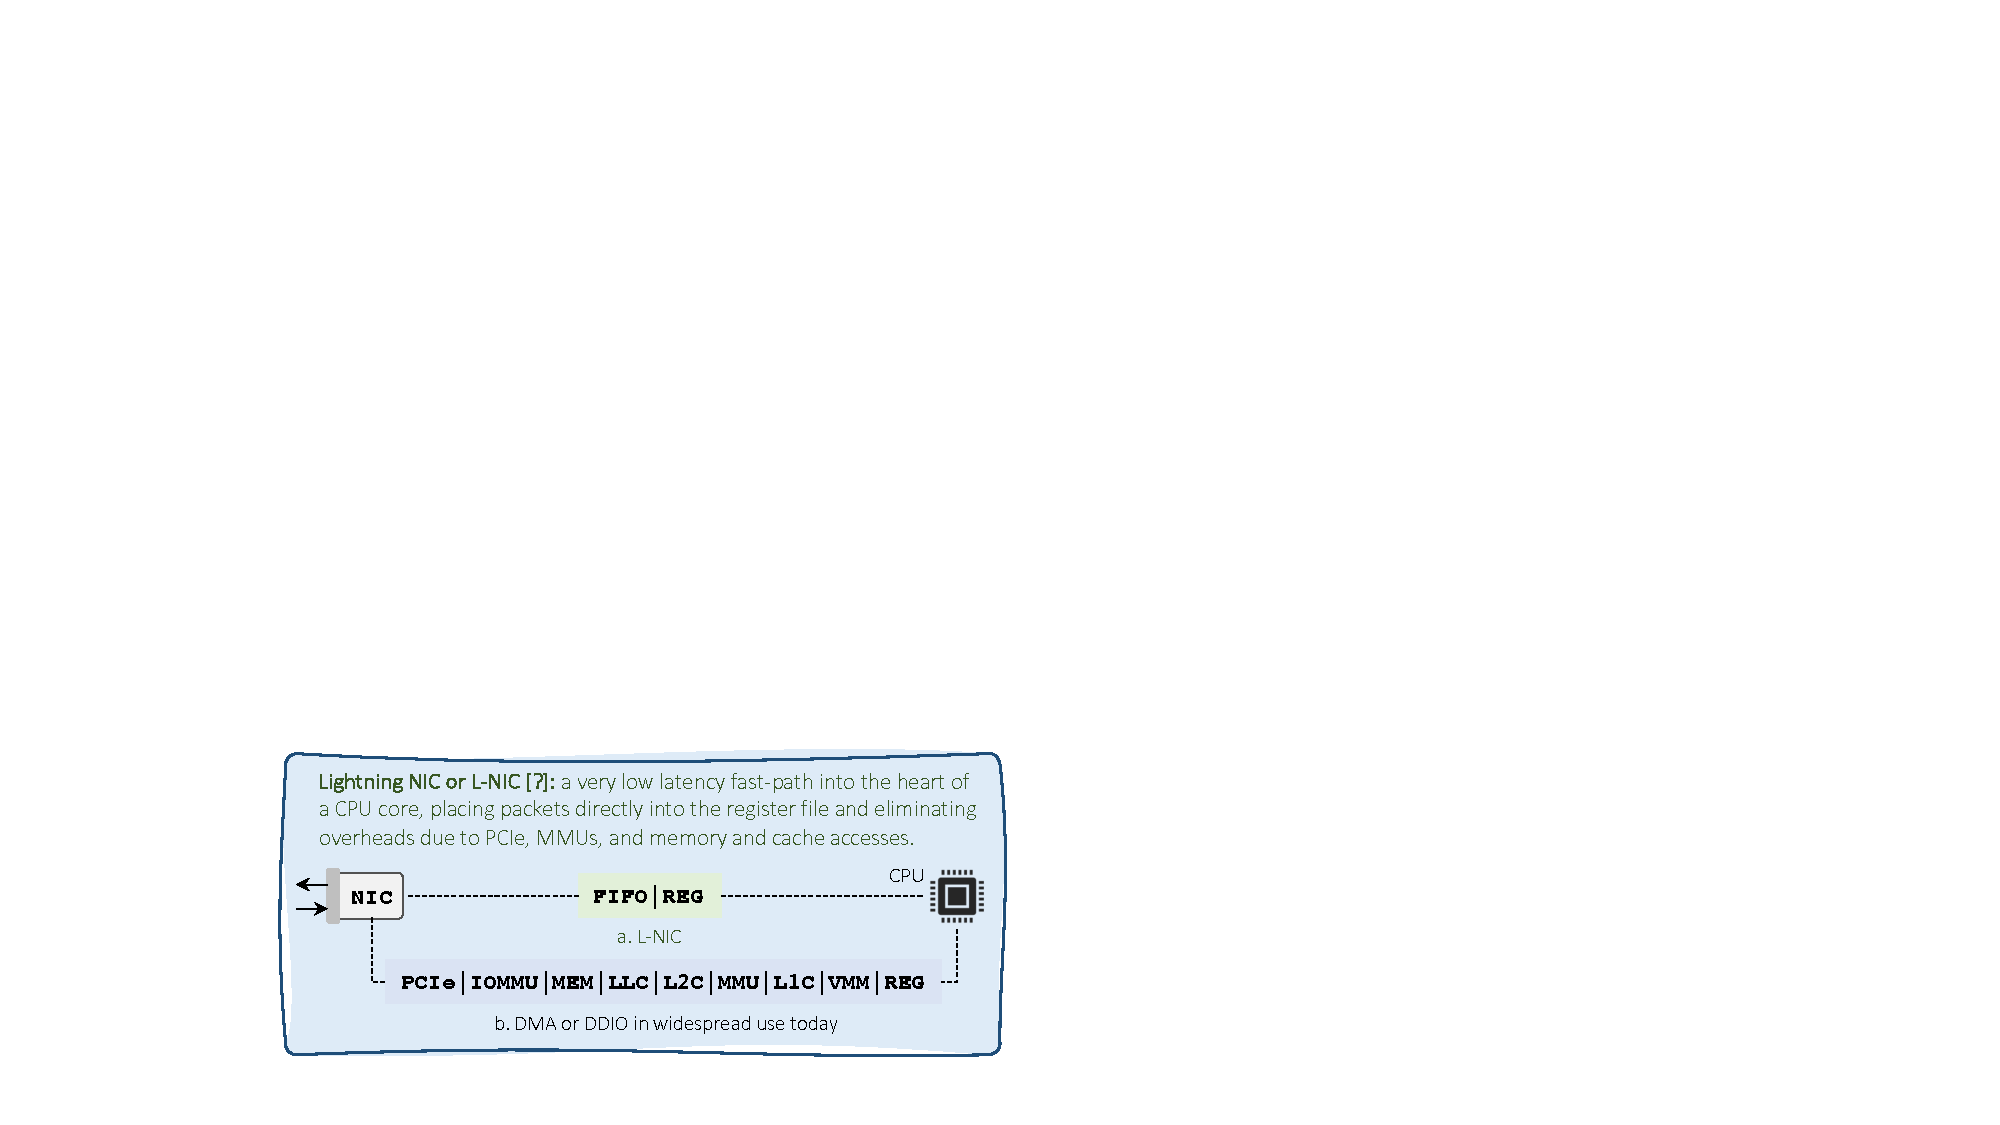
\includegraphics[width=\linewidth]{./figures/lnic-fbox}
  \label{fig:lnic-fbox}
\end{figure}

More generally, consider a distributed application consisting of $N$ potentially parallelizable tasks, each of which can be executed locally (in $x$ $\mu$s) or on a remote core via RPC (in $r \cdot x$ $\mu$s, where $r \ge 1$). 
If the degree of parallelism, $K$, is the number of issued RPCs (\ie, the number of remote cores), we minimize job-completion time when $(N - K)\cdot x = r \cdot x$ (\ie, $K = N - r$). 
Further increasing the degree of parallelism, $K$, yields no benefit; if we send more RPCs, the local core just sits idle waiting for the RPCs to complete. 
For example, if $r = 10$ (\ie, RPCs take 10 times as long as local execution) then we should send $N-10$ RPCs while executing 10 tasks locally. 
If we reduce latency so that $r=1$, the total job-completion time is reduced by 90\%.  

In practice, RPC completion times, $f_i$, are not fixed, but characterized by a probability distribution, $f_i \in \mathcal{F}$. 
The total job completion time is $(N - K) \cdot x =\max{f_i}$ where $1\le i \le K$. Thus, if we want to improve performance, we must reduce the RPC tail latency ($\max{f_i}$). 
This observation is not new and has been the motivation for much recent work~\cite{shinjuku, shenango, rpcvalet}. 

\begin{figure}
  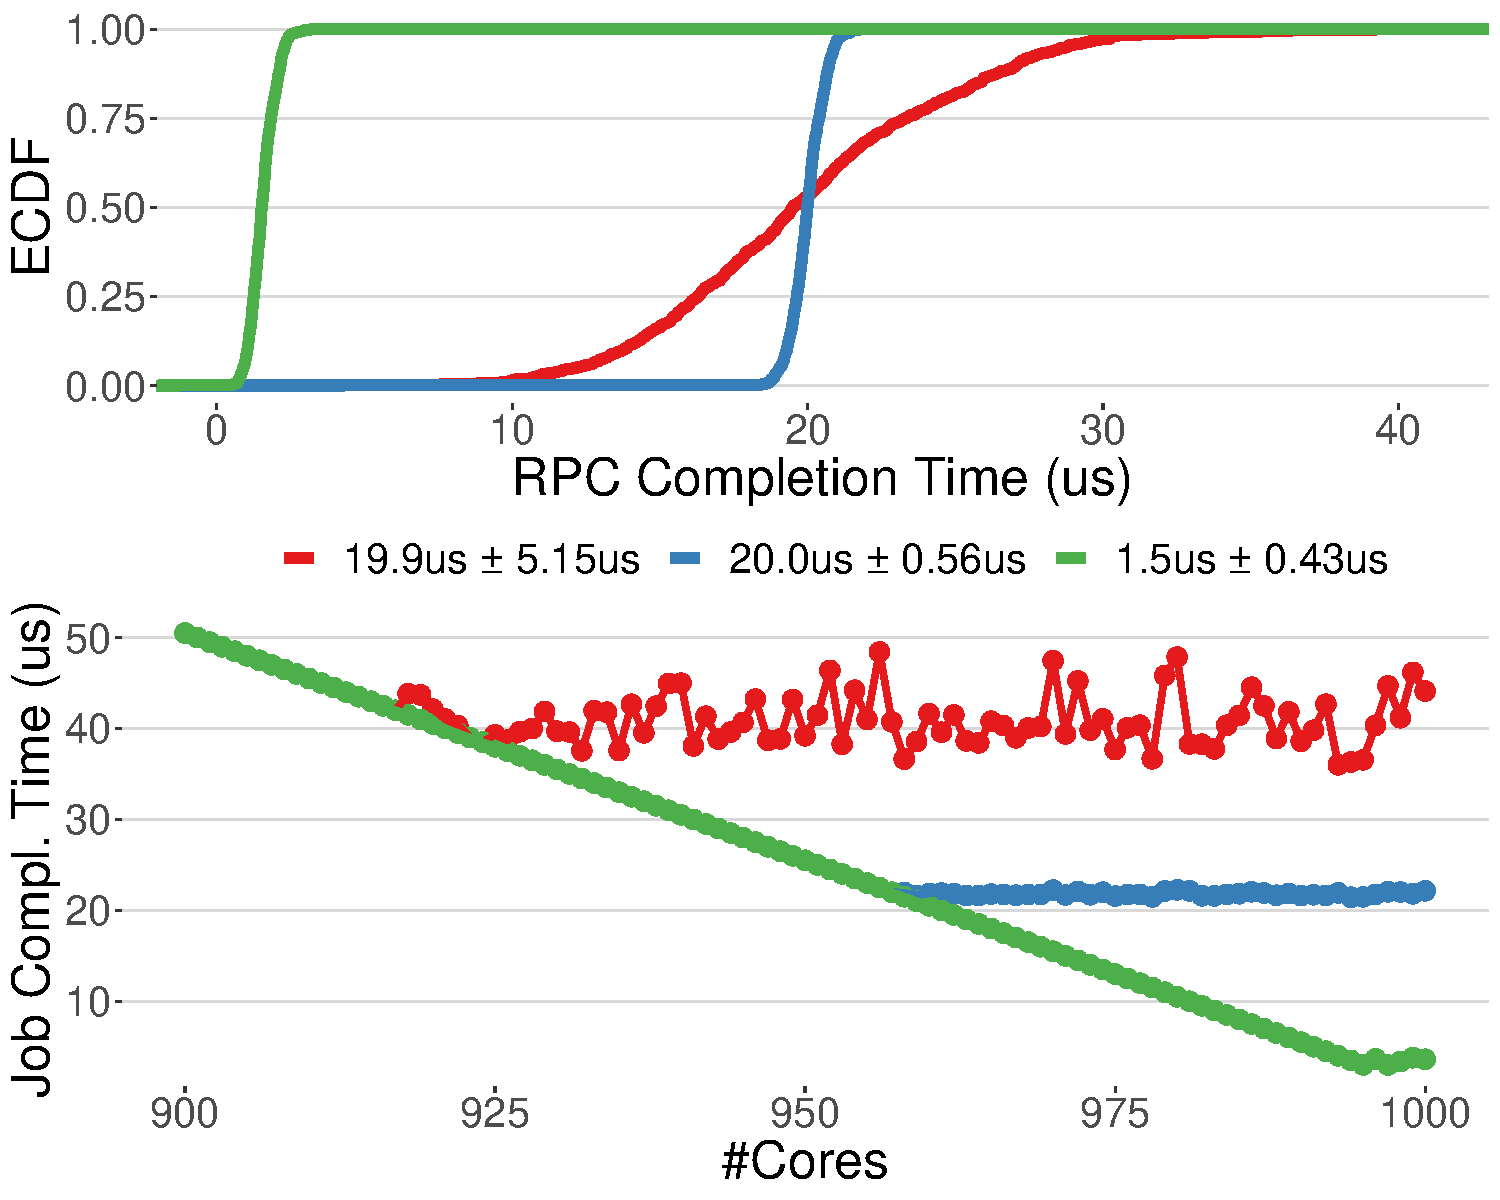
\includegraphics[width=0.9\linewidth]{./figures/nano-comptime}
  \caption{Total job completion time of an example application with 1000 independent tasks (each with \SI{500}{ns} processing time) for varying number of cores (\ie, one per RPC) under different RPC completion time distributions.}
  \label{fig:nanoservice-sim}
\end{figure}

The goal of our research is to design, build and evaluate a domain-specific processor, which we call a {\em \name{}}, optimized for minimizing the completion time of highly parallel, compute-intensive jobs. The \name{} is designed for massive scale-out computing. 
Specifically, millions of \name{}s could be deployed to run {\em nanoservices}: highly distributed, compute-intensive applications that process RPC requests in under \SI{1}{\mu s} using fine-grained, cache-resident threads.

If we are to minimize the average and tail latency of an RPC, we must minimize the latency at every step of the way. 
Starting from when a CPU thread issues an RPC, we must minimize latency through the network stack, through the cache, DRAM and DMA subsystem, through the NIC and onto the wire; across Ethernet links and through switches; and then from the destination NIC through the DMA, DRAM, and cache subsystem; through the network stack, and then wait for the RPC request's target thread to be scheduled for execution by the operating system and for the application to read and process the request.
Most prior work has focused on one aspect of an RPC's latency--for example, low-latency transport layers~\cite{homa, ndp, pfabric} to reduce network congestion and minimize latency through switches, or thread scheduling to make sure an incoming RPC request starts executing promptly~\cite{shinjuku, shenango}. 
Our goal is to reduce RPC response times by at least an order of magnitude, from tens or hundreds of microseconds down to approximately \SI{1}{\mu s}. 
This is mostly a networking problem, and leads us to tackle three questions:

\begin{enumerate}[topsep=0.4\baselineskip, leftmargin=20pt]
    \item {\bf Minimizing {\em average} RPC completion time:} How can we minimize the time that a network message spends between the wire and an application thread?
    This requires minimizing the time through hardware and software. Our approach is to build upon the extremely low-latency {\em Lightning NIC} (L-NIC), described in~\cite{lnic}, in which messages bypass the traditional networking stack, as well as the DMA, DRAM and cache hierarchy entirely, and are placed directly into the CPU register file.
    An arriving RPC can start execution in under \SI{100}{ns} (not including the MAC). 
    \item {\bf Minimizing {\em tail} RPC completion time:} How can we limit resource contention for the CPU, memory and network, and minimize the cost of context switching between threads?
    These are the primary causes of variance, and hence tail RPC completion times.
    Our approach is to design a thread scheduler into the NIC hardware, as well as to enable the NIC to implement a very low latency hardware transport layer~\cite{homa,ndp}.
    \item {\bf Making it practical:} How can such an extreme approach to hardware and software be practically deployed, with minimal disruption? 
    We have designed a hardware prototype, based on a RISC-V CPU~\cite{rocket-chip}, including a \SI{100}{Gb/s} Ethernet L-NIC CPU interface and a hardware thread scheduler, and we report performance results for real nanoservice applications.
\end{enumerate}

\Cref{fig:nanoservice-sim}, while based on synthetic numbers, illustrates what we aim to achieve.
The first graph shows various distributions of RPC completion times. 
The red graph is intended to be representative of the current state-of-the-art RPC completion times~\cite{eRPC}. The blue graph demonstrates the impact on total application runtime when the standard deviation of the RPC completion time distribution is reduced by an order of magnitude.
If we can drive down the average {\em and} the standard deviation, represented by the green line, then the job-completion time falls linearly as we add cores, until eventually the per-RPC overhead limits parallelism.

In summary, we make the following contributions:
\begin{itemize}[topsep=0.4\baselineskip, leftmargin=20pt]
    \item A new compute framework, called nanoservices (\S\ref{sec:nanoservices}), for highly parallelizable, compute-intensive distributed applications.
    \item The design and implementation of a \name{} (\S\ref{sec:nanoPU}) with a \SI{100}{Gb/s} NIC datapath (\S\ref{ssec:nic-datapath}), a message-based interface directly between the NIC and CPU register file (\S\ref{ssec:niccore-interface}) and a NIC-driven thread scheduler (\S\ref{ssec:thread-scheduler}).
    \item An overview of the hardware mechanisms to support a low-latency transport protocol on the NIC (\S\ref{ssec:nic-transport}).
    \item An open-source \name{} prototype (\S\ref{sec:prototype}), based on a RISC-V Rocket core~\cite{rocket-chip}.
    \item An evaluation of our \name{} prototype against a traditional RISC-V CPU with a DMA-based NIC, for a suite of nanoservice applications (\S\ref{sec:evaluation}). 
    Our evaluation demonstrates that \name{} reduces both average and tail RPC-completion times by about 2--10$\times$ and $20\times$, respectively.
\end{itemize}

\paragraph{Ethics} This work does not raise any ethical issues.

%%% Original Intro (2/7/20) %%%
% \section{Introduction}
% Cloud data centers allow thousands of client applications to share millions of CPU cores.
% Many of these client applications harness CPU cores using {\em coarse}-grained parallelism, such as MapReduce~\cite{mapreduce-google}, Hadoop~\cite{apache-hadoop} and client-server web applications.
% Other, more specialized applications use {\em fine}-grained parallelism to employ hundreds of thousands of CPUs (\eg, search~\cite{barroso2003web}, HPC~\cite{ibm-hpc}).
% It is well-known to be difficult to write applications using fine-grained parallelism, and so the technique is generally reserved as a last resort, for when applications must respond quickly (\eg, search or ads), or must complete in a reasonable time (\eg, a large HPC physical simulation~\cite{changa, blue-gene-l, barnes-hut} or overnight ML training~\cite{tensorflow}).
% Recently, as applications have grown ever larger (\eg, mushrooming ML training data, big data analytics, and social media), the speed of individual cores has grown ever more slowly~\cite{hp-comp-arch}.
% Increased parallelism is inevitable.

% Some recent products and open-source projects have used fine-grain modules, deployed as microservices (\eg, AWS Lambda~\cite{aws-lambda}, Azure Serverless Computing~\cite{azure-functions}, Google Cloud Functions~\cite{gcloud-functions}, and OpenFaaS~\cite{openfaas}) to demonstrate impressive speedup of parallel applications, including video encoding~\cite{ExCamera}, video compression~\cite{sprocket}, and face recognition~\cite{cirrus}, by successfully employing thousands of CPU cores in parallel.
% But, as we will see, this level of parallelism still yields far from the fastest possible execution time.

% In the limit, if we segment an application into its smallest, indivisible software modules, {\em and if communication is instantaneous}, then an application can complete in the execution time of the longest sequence of serially-dependent modules.
% But, communication is not instantaneous---far from it. 
% Many researchers have reported the (surprisingly) high communication latency between two cores, \eg, a request-response time of \SI{0.7}{ms}~\cite{eRPC, perfkit-grpc}.
% Intuitively, if it takes \SI{0.7}{ms} to ask another CPU to execute a function, then it is only worth doing if we have more than \SI{0.7}{ms} of work to do; otherwise we might as well execute the code locally. 

% For example, consider a physical simulation of one million objects, where each object needs to update its ten neighbors each time it moves. 
% If each object executes \SI{10}{\mu s} of code to calculate its move (about 40,000 instructions on a modern CPU), but takes \SI{1}{ms} to tell its neighbors, then latency dominates the computation, and it makes sense for 10--100 objects to share one core. 
% If instead, an RPC call could complete in less than \SI{1}{\mu s}, then it makes sense for each object to run on its own core, and the simulation can complete one hundred times sooner. 

% \begin{figure}[t]
%   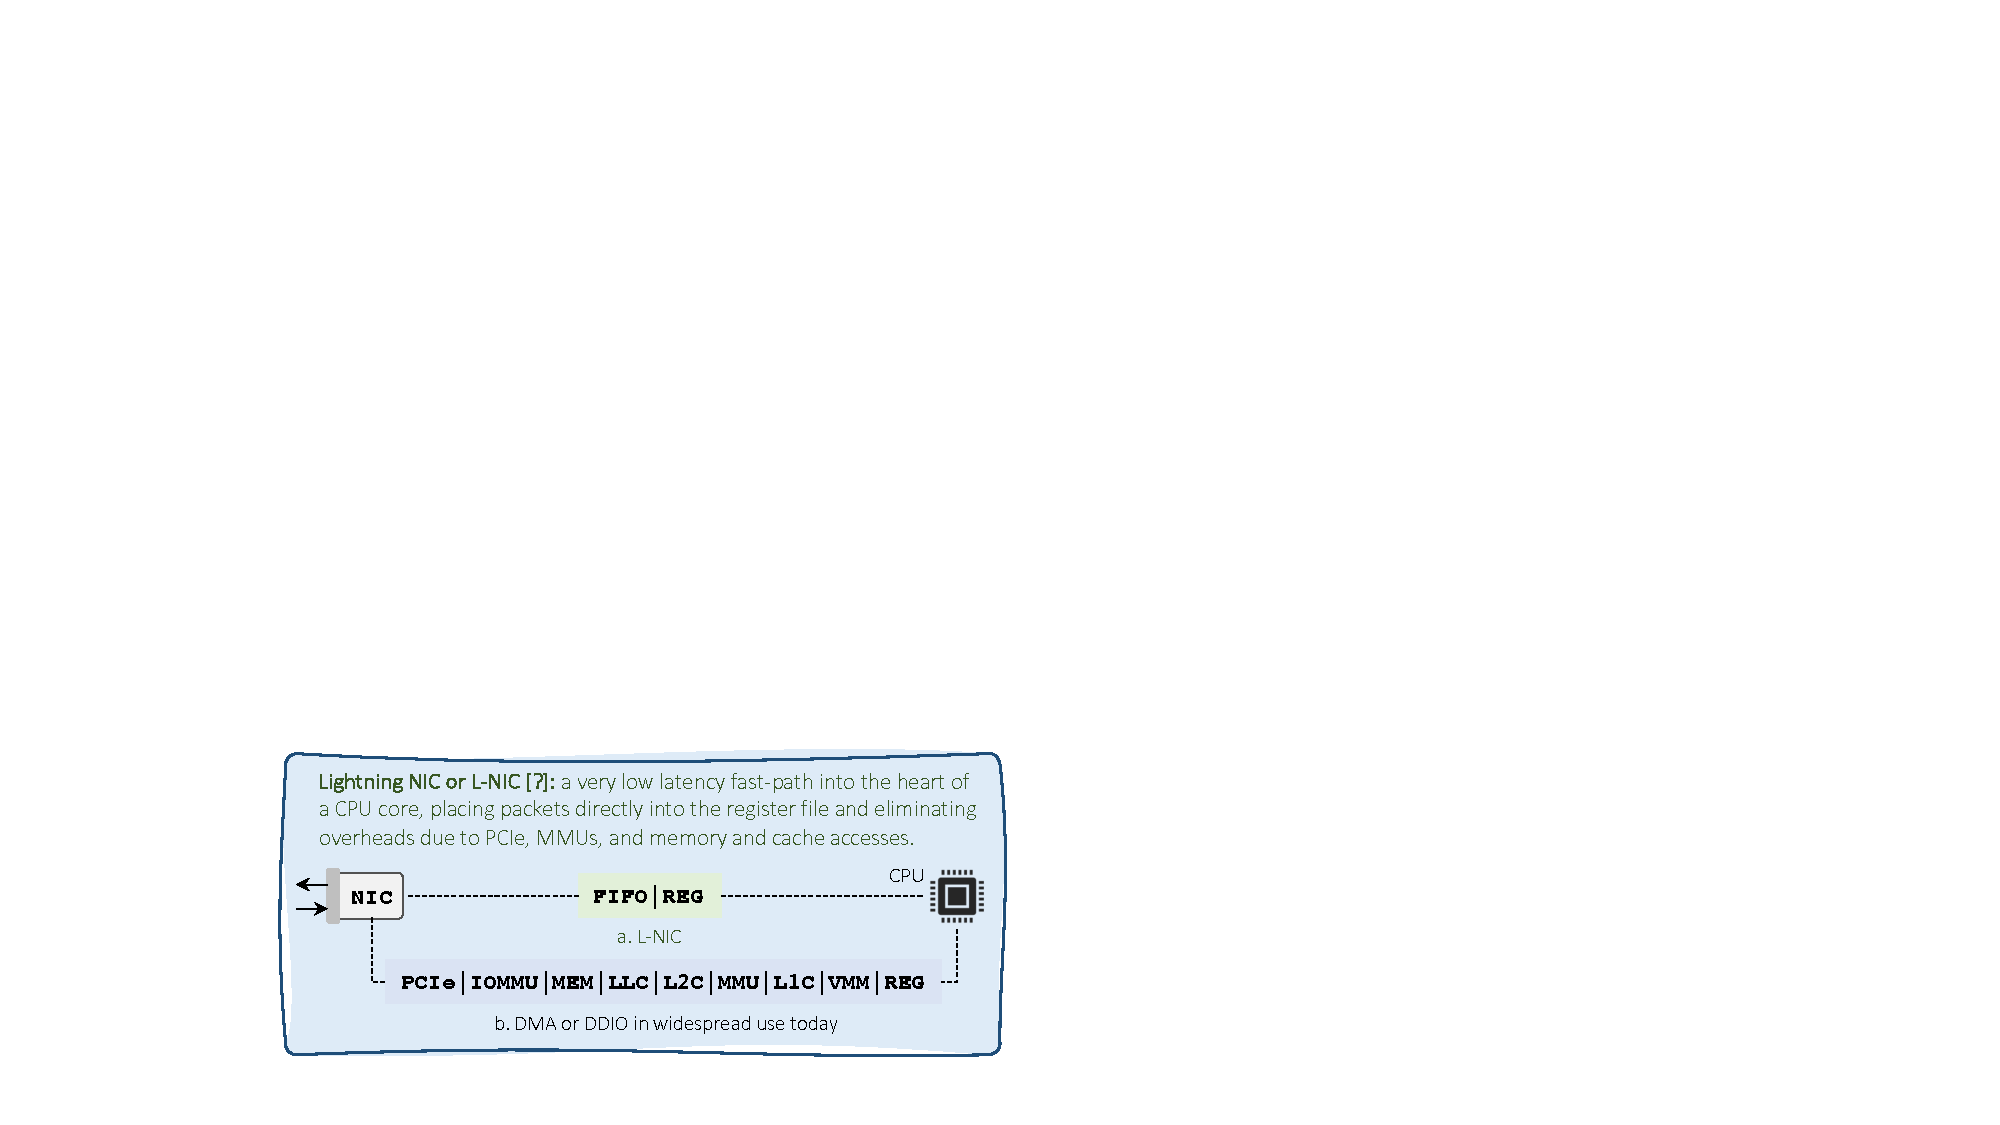
\includegraphics[width=\linewidth]{./figures/lnic-fbox}
%   \label{fig:lnic-fbox}
% \end{figure}
% \shahbaz{add missing citations once the paper is ready.}

% More generally, consider a distributed application consisting of $N$ potentially parallelizable tasks, each of which can be executed locally (in $x$ $\mu$s) or on a remote core via RPC (in $r \cdot x$ $\mu$s, where $r \ge 1$). 
% If the degree of parallelism, $K$, is the number of issued RPCs (\ie, the number of remote cores), we minimize job-completion time when $(N - K)\cdot x = r \cdot x$ (\ie, $K = N - r$). 
% Further increasing the degree of parallelism, $K$, yields no benefit; if we send more RPCs, the local core just sits idle waiting for the RPCs to complete. 
% For example, if $r = 10$ (\ie, RPCs take 10 times as long as local execution) then we should send $N-10$ RPCs while executing 10 tasks locally. 
% If we reduce latency so that $r=1$, the total job-completion time is reduced by 90\%.  

% In practice, RPC completion times, $f_i$, are not fixed, but characterized by a probability distribution, $f_i \in \mathcal{F}$. 
% The total job completion time is $(N - K) \cdot x =\max{f_i}$ where $1\le i \le K$. Thus, if we want to improve performance, we must reduce the RPC tail latency ($\max{f_i}$). 
% This observation is not new and has been the motivation for much recent work~\cite{shinjuku, shenango, rpcvalet}. 

% \begin{figure}
%   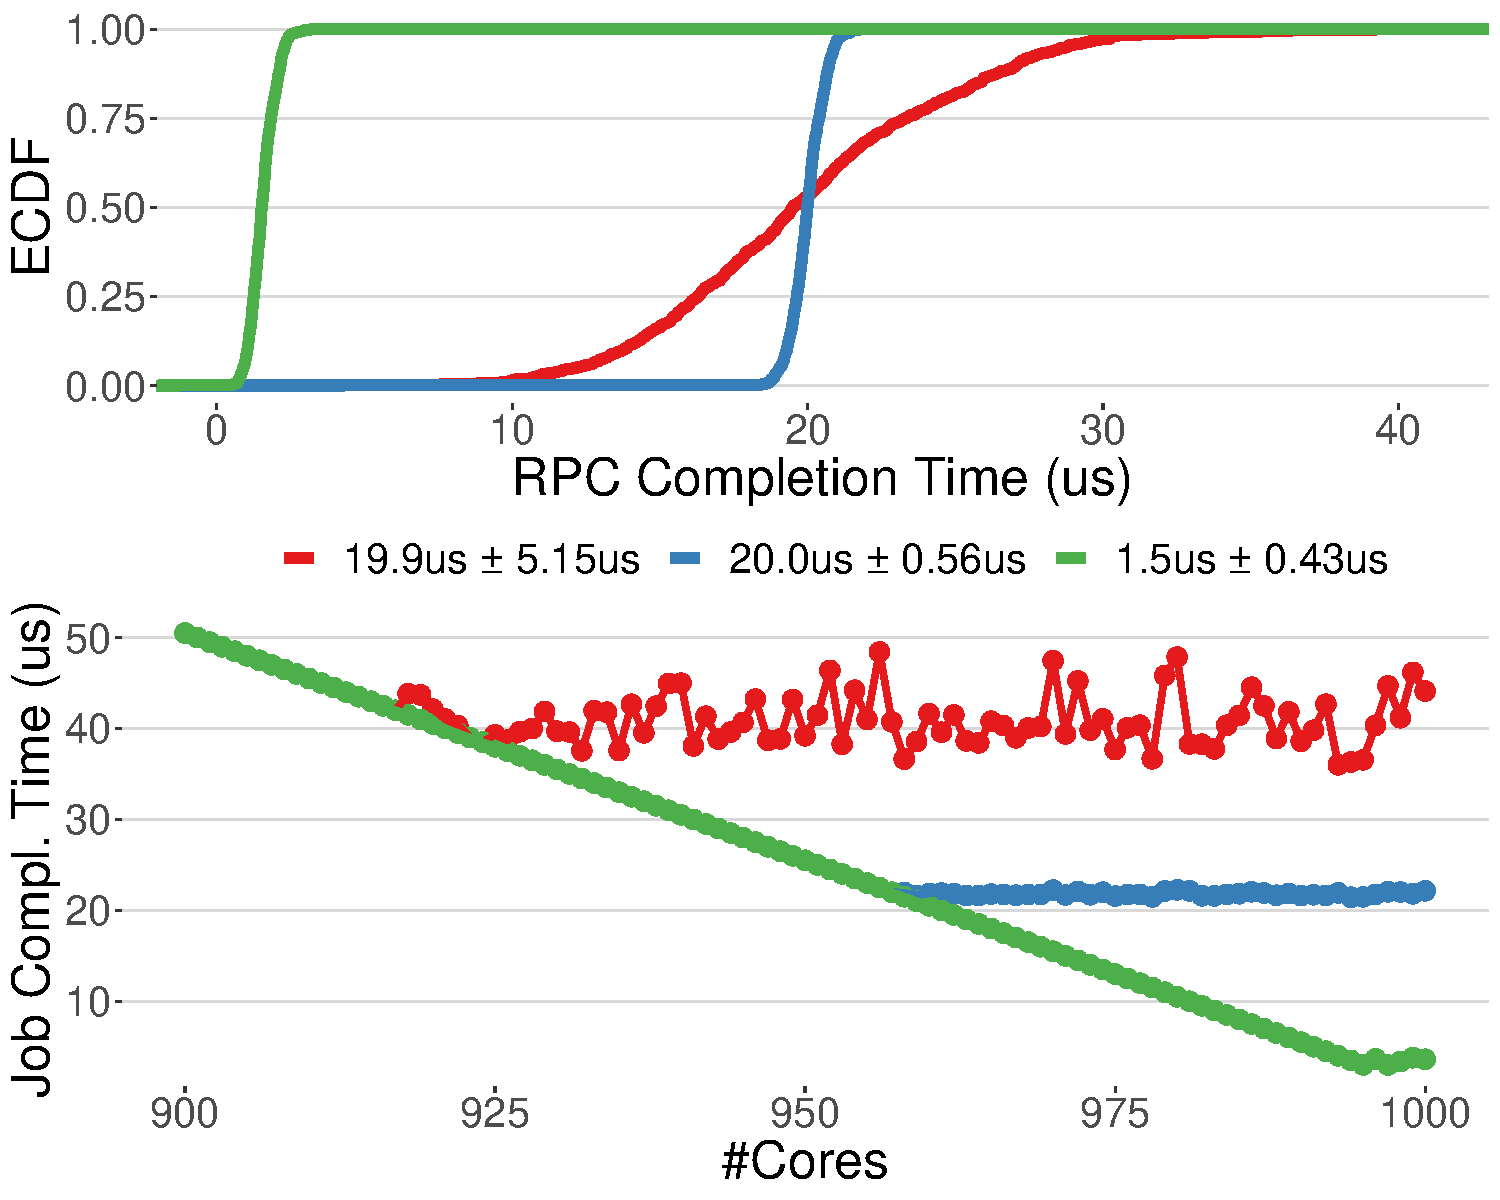
\includegraphics[width=0.9\linewidth]{./figures/nano-comptime}
%   \caption{Total job completion time of an example application with 1000 independent tasks (each with \SI{500}{\mu s} processing time) for varying number of cores (\ie, one per RPC) under different RPC completion time distributions.}
%   \label{fig:nanoservice-sim}
% \end{figure}

% The goal of our research is to design, build, and evaluate a domain-specific processor, which we call a {\em \name{}}, optimized for minimizing the completion time of highly-parallel, compute-intensive jobs. The \name{} is designed for massive scale-out computing. 
% Specifically, millions of \name{}s could be deployed to run {\em nanoservices}: highly distributed, compute-intensive applications that process RPC requests in under \SI{1}{\mu s} using fine-grained, cache-resident threads.

% If we are to minimize the average and tail latency of an RPC, we must minimize the latency at every step of the way. 
% Starting from when a CPU thread issues an RPC, we must minimize latency through the network stack, through the cache, DRAM and DMA subsystem, through the NIC and onto the wire; across Ethernet links and through switches; and then from the destination NIC through the DMA, DRAM, and cache subsystem; through the network stack, and then wait for the RPC request's target thread to be scheduled for execution by the operating system and for the application to read and process the request.
% Most prior work has focused on one aspect of an RPC's latency--for example, low-latency transport layers~\cite{homa, ndp, pfabric} to reduce network congestion and minimize latency through switches, or thread scheduling to make sure an incoming RPC request starts executing promptly~\cite{shinjuku, shenango}. 
% Our goal is to reduce RPC response times by at least an order of magnitude from tens or hundreds of microseconds down to approximately \SI{1}{\mu s}. 
% This is mostly a networking problem, and leads us to tackle three questions:

% \begin{enumerate}[topsep=0.4\baselineskip, leftmargin=20pt]
%     \item {\bf Minimizing {\em average} RPC completion time:} How can we minimize the time that a network message spends between the wire and an application thread?
%     This requires minimizing the time through hardware and software. Our approach is to build upon the extremely low-latency {\em Lightning NIC} (L-NIC), described in~\cite{lnic}, in which messages bypass the traditional networking stack, as well as the DMA, DRAM and cache hierarchy entirely, and are placed directly into the CPU register file.
%     An arriving RPC can start execution in under \SI{100}{ns} (not including the MAC). 
%     \item {\bf Minimizing {\em tail} RPC completion time:} How can we limit resource contention for the CPU, memory and network, and minimize the cost of context switching between threads?
%     These are the primary causes of variance and hence tail RPC completion times.
%     Our approach is to design a thread scheduler into the NIC hardware, as well as to enable the NIC to implement a very low latency hardware transport layer~\cite{homa,ndp}.
%     \item {\bf Making it practical:} How can such an extreme approach to hardware and software be practically deployed, with minimal disruption? 
%     We have designed a hardware prototype, based on a RISC-V CPU~\cite{rocket-chip}, including a \SI{100}{Gb/s} Ethernet L-NIC CPU interface and a hardware thread scheduler, and we report performance results for real nanoservice applications.
% \end{enumerate}

% \Cref{fig:nanoservice-sim}, while based on synthetic numbers, illustrates what we aim to achieve.
% The first graph shows various distributions of RPC completion times. 
% The red graph is intended to be representative of the current state-of-the-art RPC completion times~\cite{eRPC}. The blue graph demonstrates the impact on total application runtime when the standard deviation of the RPC completion time distribution is reduced by an order of magnitude.
% If we can drive down the average {\em and} the standard deviation, represented by the green line, then the job-completion time falls linearly as we add cores, until eventually the per-RPC overhead limits parallelism.

% In summary, we make the following contributions:
% \begin{itemize}[topsep=0.4\baselineskip, leftmargin=20pt]
%     \item A new compute framework, called nanoservices (\S\ref{sec:nanoservices}), for highly parallelizable, compute-intensive distributed applications.
%     \item The design and implementation of a \name{} (\S\ref{sec:nanoPU}) with a \SI{100}{Gb/s} NIC datapath (\S\ref{ssec:nic-datapath}), a message-based interface directly between the NIC and CPU register file (\S\ref{ssec:niccore-interface}) and a NIC-driven thread scheduler (\S\ref{ssec:thread-scheduler}).
%     \item An overview of the hardware mechanisms to support a low-latency transport protocol on the NIC (\S\ref{ssec:nic-transport}).
%     \item An open-source \name{} prototype (\S\ref{sec:prototype}), based on a RISC-V Rocket Core~\cite{rocket-chip}.
%     \item An evaluation of our \name{} prototype against a traditional RISC-V CPU with a DMA-based NIC, for a suite of nanoservice applications (\S\ref{sec:evaluation}). 
%     Our evaluation demonstrates that \name{} reduces both average and tail RPC-completion times by about 2--10$\times$ and $20\times$, respectively.
% \end{itemize}